\let\negmedspace\undefined
\let\negthickspace\undefined
\documentclass[journal]{IEEEtran}
\usepackage[a5paper, margin=10mm, onecolumn]{geometry}
\usepackage{lmodern} % Ensure lmodern is loaded for pdflatex
\usepackage{tfrupee} % Include tfrupee package

\setlength{\headheight}{1cm} % Set the height of the header box
\setlength{\headsep}{0mm}     % Set the distance between the header box and the top of the text

\usepackage{gvv-book}
\usepackage{gvv}
\usepackage{cite}
\usepackage{amsmath,amssymb,amsfonts,amsthm}
\usepackage{algorithmic}
\usepackage{graphicx}
\usepackage{textcomp}
\usepackage{xcolor}
\usepackage{txfonts}
\usepackage{listings}
\usepackage{enumitem}
\usepackage{mathtools}
\usepackage{gensymb}
\usepackage{comment}
\usepackage[breaklinks=true]{hyperref}
\usepackage{tkz-euclide} 
\usepackage{listings}
\usepackage{gvv}                                        
\def\inputGnumericTable{}                                 
\usepackage[latin1]{inputenc}                                
\usepackage{color}                                            
\usepackage{array}                                            
\usepackage{longtable}                                       
\usepackage{calc}                                             
\usepackage{multirow}                                         
\usepackage{hhline}                                           
\usepackage{ifthen}                                           
\usepackage{lscape}
\begin{document}

    

\section*{General Aptitude (GA)}

\begin{enumerate}              
    \item An apple costs Rs. 10. An onion costs Rs.8 Select the most suitable sentence with respect to grammar and usage.
    
    \begin{enumerate}              
   
        \item The price of an apple is greater than an onion.
        \item The price of an apple is more than onion.
        \item The price of an apple is greater than that of an onion.
        \item Apples are more costlier than onions.
      
     \end{enumerate}              
    
    \hfill{\brak{\text{GATE PE 2016}}}
    
    \item The Buddha said, "Holding on to anger is like grasping a hot coal with the intent of throwing it at someone else; you are the one who gets burnt."
    
    Select the word below which is closest in meaning to the word underlined above.
    
    \begin{enumerate} \begin{multicols}{2}              
   
        \item burning 
        \item igniting 
        \item clutching 
        \item flinging
    
    \end{multicols} \end{enumerate}              
    
    \hfill{\brak{\text{GATE PE 2016}}}
    
    \item M has a son Q and a daughter R. He has no other children. E is the mother of P and daughter-in-law of M. How is P related to M?
    
    \begin{enumerate} \begin{multicols}{2}              
    
        \item P is the son-in-law of M. 
        \item P is the grandchild of M.
        \item P is the daughter-in law of M. 
        \item P is the grandfather of M.
        
    \end{multicols} \end{enumerate}              
    
    \hfill{\brak{\text{GATE PE 2016}}}
    
    \item The number that least fits this set: $(324, 441, 97, 64)$ is .
    
    \begin{enumerate} \begin{multicols}{2}               
        \item 324 
        \item 441 
        \item 97 
        \item 64
        
    \end{multicols} \end{enumerate}              
    
    \hfill{\brak{\text{GATE PE 2016}}}
    
    \item It takes 10 s and 15 s, respectively, for two trains travelling at different constant speeds to completely pass a telegraph post. The length of the first train is 120 m and that of the second train is 150 m. The magnitude of the difference in the speeds of the two trains \brak{\text{in m/s}} is 
    
    \begin{enumerate} \begin{multicols}{2}              
        \item 2.0 
        \item 10.0 
        \item 12.0 
        \item 22.0
    \end{multicols} \end{enumerate}              
    
    \hfill{\brak{\text{GATE PE 2016}}}
         



            
    \item The velocity V of a vehicle along a straight line is measured in m/s and plotted as shown with respect to time in seconds. At the end of the 7 seconds, how much will the odometer reading increase by \brak{\text{in m}}?
   \begin{figure}
       \centering
       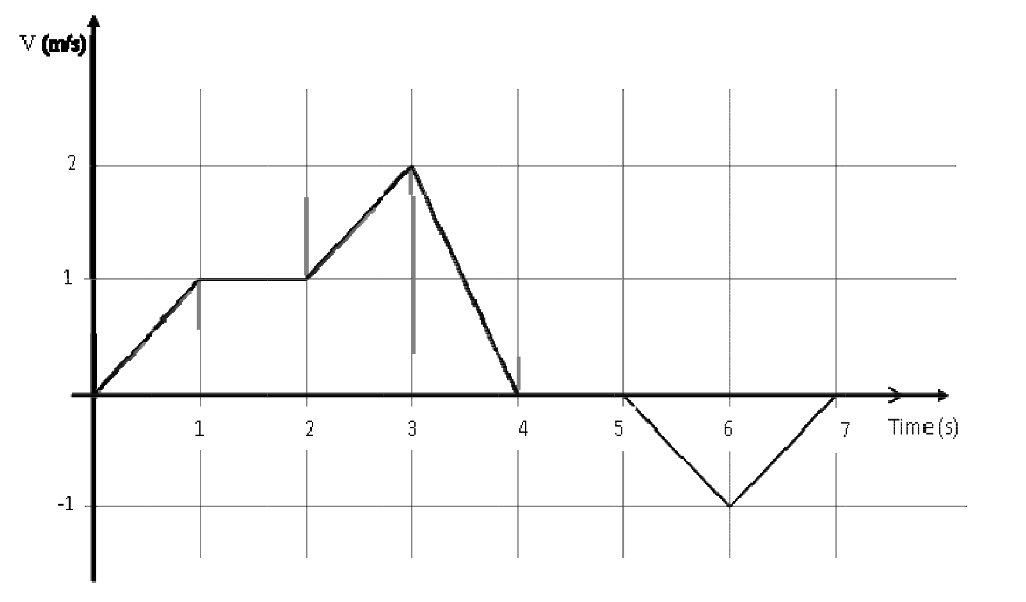
\includegraphics[width=0.5\linewidth]{figs/i 1.jpeg}
       \caption{Caption}
       \label{fig:placeholder}
   \end{figure}
    
    
    \begin{enumerate} \begin{multicols}{2}              
     
        \item 0    
        \item 3    
        \item 4    
        \item 5
    \end{multicols} \end{enumerate}              
    
    \hfill{\brak{\text{GATE PE 2016}}}
    
 \item The overwhelming number of people infected with rabies in India has been flagged by the World Health Organization as a source of concern. It is estimated that inoculating 70\% of pets and stray dogs against rabies can lead to a significant reduction in the number of people infected with rabies.
    
    Which of the following can be logically inferred from the above sentences?
    
    \begin{enumerate}              
        \item The number of people in India infected with rabies is high.
        \item The number of people in other parts of the world who are infected with rabies is low.
        \item Rabies can be eradicated in India by vaccinating 70\% of stray dogs.
        \item Stray dogs are the main source of rabies worldwide.
    \end{enumerate}              
    
    \hfill{\brak{\text{GATE PE 2016}}}
    
    \item A flat is shared by four first year undergraduate students. They agreed to allow the oldest of them to enjoy some extra space in the flat. Manu is two months older than Sravan, who is three months younger than Trideep. Pavan is one month older than Sravan. Who should occupy the extra space in the flat?
    
    \begin{enumerate} \begin{multicols}{2}              
        \item Manu    
        \item Sravan    
        \item Trideep    
        \item Pavan
    \end{multicols} \end{enumerate}              
    
    \hfill{\brak{\text{GATE PE 2016}}}
    
    \item Find the area bounded by the lines $3x+2y=14$, $2x-3y=5$ in the first quadrant.
    
    \begin{enumerate} \begin{multicols}{2}              
        \item 14.95    
        \item 15.25    
        \item 15.70    
        \item 20.35
    \end{multicols} \end{enumerate}              
    
    \hfill{\brak{\text{GATE PE 2016}}}
    
    \item A straight line is fit to a data set $(\ln x, y)$. This line intercepts the abscissa at $\ln x = 0.1$ and has a slope of $-0.02$. What is the value of $y$ at $x = 5$ from the fit?
    
    \begin{enumerate} \begin{multicols}{2}              
        \item $-0.030$ 
        \item $-0.014$ 
        \item $0.014$ 
        \item $0.030$
    \end{multicols} \end{enumerate}              
    
    \hfill{\brak{\text{GATE PE 2016}}}
 
\section*{Petroleum Engineering (PE)}
    \item The value of   
   \begin{align}
 \lim_{x \to 0} \left( \frac{e^x - 1}{\sin x} \right)      
   \end{align} 
    is equal to 
    \hfill{\brak{\text{GATE PE 2016}}}
    
    \item The function 
    \begin{align}
     f(x) = \frac{1}{1 + |x|}   
    \end{align}
      is
    \begin{enumerate} \begin{multicols}{2}              
        \item continuous and differentiable.
        \item continuous but not differentiable.
        \item not continuous but differentiable.
        \item not continuous and not differentiable.
    \end{multicols} \end{enumerate}              
    
    \hfill{\brak{\text{GATE PE 2016}}}
    
    \item The value of the definite integral 
    \begin{align}
      \int_1^e (\ln x) \, dx   
    \end{align}
     is equal to . 
    \hfill{\brak{\text{GATE PE 2016}}}
    \item For a complex number  
    \begin{align}
         Z = \left( \frac{1}{2} + \frac{\sqrt{3}}{2} i \right) 
    \end{align}
   , the value of 
   \begin{align}
     Z^e   
   \end{align}
    is
    
    \begin{enumerate} \begin{multicols}{2}              
        \item $-\left( \frac{1}{2} + \frac{\sqrt{3}}{2} i \right)$ 
        \item $-1$ 
        \item $\left( \frac{1}{2} - \frac{\sqrt{3}}{2} i \right)$ 
        \item $1$
    \end{multicols} \end{enumerate}              
    
    \hfill{\brak{\text{GATE PE 2016}}}
    
    \item The Laplace transform of the function $e^{-2t}$ is
    
    \begin{enumerate} \begin{multicols}{2}              
        \item $\frac{1}{2s}$ 
        \item $\frac{2}{s}$ 
        \item $\frac{1}{s + 2}$ 
        \item $e^{-2s}$
    \end{multicols} \end{enumerate}              
    
    \hfill{\brak{\text{GATE PE 2016}}}
    
    \item Which of the following is preferred fast neutron source in neutron logging?
    \begin{enumerate} \begin{multicols}{2}              
        \item Americium-Beryllium
        \item Radium-Beryllium
        \item Deuterium-Tritium
        \item Thorium-Beryllium
    \end{multicols} \end{enumerate}              
    \hfill{\brak{\text{GATE PE 2016}}}
    \item Using the gamma ray log given in the figure, the shaliness index for point S is .
    \begin{figure}
        \centering
        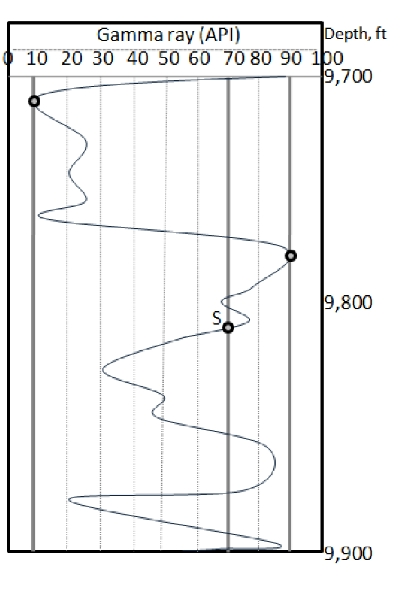
\includegraphics[width=0.5\columnwidth]{figs/i 2.jpeg}
        \caption{}
        \label{fig:placeholder}
    \end{figure}

    
    \hfill{\brak{\text{GATE PE 2016}}}
    
    \item Identify the logging device that is based on the concept of longitudinal and transverse relaxation times.
    
    \begin{enumerate} \begin{multicols}{2}              
        \item Thermal neutron decay  
        \item Induced gamma ray spectroscopy  
        \item Neutron  
        \item Nuclear Magnetic Resonance \brak{NMR}
    \end{multicols} \end{enumerate}              
    
    \hfill{\brak{\text{GATE PE 2016}}}
    
    \item The three main stages of evolution of organic matter in sediments are Catagenesis \brak{C}, Diagenesis \brak{D} and Metagenesis \brak{M}. Their chronological order is  
    
    \begin{enumerate} \begin{multicols}{2}              
        \item D - C - M  
        \item C - D - M  
        \item D - M - C  
        \item C - M - D
    \end{multicols} \end{enumerate}              
    
    \hfill{\brak{\text{GATE PE 2016}}}
    
    \item For a kick off operation, a directional well has to be drilled for an arc-length of 2500 ft to achieve an inclination of 50°.
    
    The radius of curvature will be \_\_\_\_ ft.
    
    \hfill{\brak{\text{GATE PE 2016}}}
    
    \item Which of the following is the MOST COMMON cause for a fishing job?
    
    \begin{enumerate} \begin{multicols}{2}              
        \item Differential sticking  
        \item Use of oil based mud  
        \item Lost circulation  
        \item Well kick
    \end{multicols} \end{enumerate}              
    
    \hfill{\brak{\text{GATE PE 2016}}}
    
    \item The figure shows the producing gas oil ratio \brak{GOR} behaviour with time for an oil reservoir under primary production. At initial reservoir condition, $P_b$ is the bubble point pressure of the crude oil. $P_R(t)$ represents the reservoir pressure at time 't'. Which of the following statements is TRUE?
    \begin{figure}
        \centering
        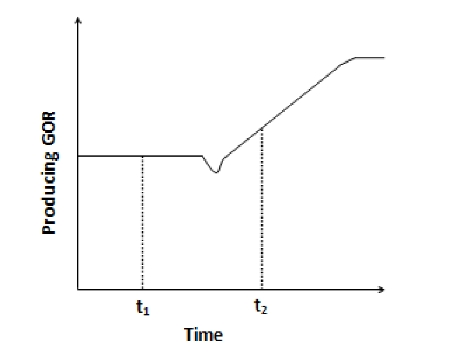
\includegraphics[width=0.5\columnwidth]{figs/i 3.jpeg}
        \caption{}
        \label{fig:placeholder}
    \end{figure}
    
    
 
    
    \begin{enumerate} \begin{multicols}{2}              
        \item $P_R(t_1) > P_b$, $P_R(t_2) > P_b$  
        \item $P_R(t_1) > P_b$, $P_R(t_2) < P_b$  
        \item $P_R(t_1) < P_b$, $P_R(t_2) > P_b$  
        \item $P_R(t_1) < P_b$, $P_R(t_2) < P_b$
    \end{multicols} \end{enumerate}              
    
    \hfill{\brak{\text{GATE PE 2016}}}
    
    \item A core, with a length of 10 cm, breadth of 4 cm and width of 4 cm, weighs 282.4 g in its dry form. The core is then saturated 100\% with brine of density 1.1 g/cm$^3$. The brine saturated core weighs 300 g.
    
    The porosity of this core sample is \_\_\_\_\_\%.
    
    \hfill{\brak{\text{GATE PE 2016}}}
    
    \item A hydraulic line of a subsurface safety valve has a fluid of specific gravity 1.2 to operate the valve. The valve closing pressure is 1,200 psia and the recommended safety margin is 200 psia.
    
    The maximum depth at which the valve can be positioned is \_\_\_\_\_ ft.
    
    \hfill{\brak{\text{GATE PE 2016}}}
    
    \item A sucker rod pump unit is designated by C-228D-200-74. Here, 'D' represents
    
    \begin{enumerate} \begin{multicols}{2}              
        \item double reduction gear box.  
        \item diameter of sucker rod.  
        \item diameter of plunger.  
        \item stroke length.
    \end{multicols} \end{enumerate}              
    
    \hfill{\brak{\text{GATE PE 2016}}}
    
    \item The three translational motions for a floating vessel are
    
    \begin{enumerate} \begin{multicols}{2}              
        \item Roll-Pitch-Yaw.  
        \item Heave-Pitch-Sway.  
        \item Surge-Sway-Heave.  
        \item Roll-Sway-Heave.
    \end{multicols} \end{enumerate}              
    
    \hfill{\brak{\text{GATE PE 2016}}}
    
    \item Jack-up rigs are typically used for off-shore drilling when the water depth is in the range
    
    \begin{enumerate} \begin{multicols}{2}              
        \item $<$ 25 ft  
        \item 50 $-$ 500 ft  
        \item 1000 $-$ 2000 ft  
        \item $>$ 2000 ft
    \end{multicols} \end{enumerate}              
    
    \hfill{\brak{\text{GATE PE 2016}}}
    
    \item Interference tests can be used for
    
    I. determining communication between two or more wells.
    II. mature oil wells having skin damage.
    III. determining permeability in tested wells.
    IV. providing inputs for secondary and tertiary oil recovery methods
    
    \begin{enumerate} \begin{multicols}{2}              
        \item only I and II  
        \item only I, II and IV  
        \item only II, III and IV  
        \item I, II, III and IV
    \end{multicols} \end{enumerate}              
    
    \hfill{\brak{\text{GATE PE 2016}}}
    
    \item For an effective hydraulically-fractured well, the skin factor would GENERALLY be
    
    \begin{enumerate} \begin{multicols}{2}              
        \item negative.  
        \item positive.  
        \item zero.  
        \item indeterminate.
    \end{multicols} \end{enumerate}              
    
    \hfill{\brak{\text{GATE PE 2016}}}
    
    \item The maximum discharge limit of oil and grease in a marine coastal area as per Environmental (protection) Rules, 1986 in India is
    
    \begin{enumerate} \begin{multicols}{2}              
        \item 0.1 mg/L.  
        \item 20 mg/L.  
        \item 500 mg/L.  
        \item 4000 mg/L.
    \end{multicols} \end{enumerate}              
    
    \hfill{\brak{\text{GATE PE 2016}}}
    
    \item Which of the following gases is NOT responsible for global warming?
    
    \begin{enumerate} \begin{multicols}{2}              
        \item Carbon dioxide  
        \item Methane  
        \item Water vapour  
        \item Nitrogen
    \end{multicols} \end{enumerate}              
    
    \hfill{\brak{\text{GATE PE 2016}}}
    
    \item In an oil reservoir flooded with water, the volumetric sweep efficiency is 70\%. The connate water saturation in the reservoir is 0.4 and the residual oil saturation for the water flood is 0.3.
    
    The overall efficiency of the reservoir is \_\_\_\_\_\%.
    
    \hfill{\brak{\text{GATE PE 2016}}}
    
    \item Identify the pair of CORRECT statements for surfactant-micellar-polymer flooding.
    
    I. It reduces interfacial tension between crude oil and water.
    II. It influences mobility ratio unfavorably.
    III. It improves microscopic displacement efficiency.
    IV. It increases isothermal compressibility of the crude oil.
    
    \begin{enumerate} \begin{multicols}{2}              
        \item I \& II  
        \item I \& III  
        \item III \& IV  
        \item II \& IV
    \end{multicols} \end{enumerate}              
    
    \hfill{\brak{\text{GATE PE 2016}}}
    
    \item Gas hydrate forms at
    
    \begin{enumerate} \begin{multicols}{2}              
        \item low pressure and low temperature conditions.  
        \item low pressure and high temperature conditions.  
        \item high pressure and low temperature conditions.  
        \item high pressure and high temperature conditions.
    \end{multicols} \end{enumerate}              
    
    \hfill{\brak{\text{GATE PE 2016}}}
    
    \item Production of coal bed methane \brak{CBM} is based on
    
    \begin{enumerate} \begin{multicols}{2}              
        \item distillation.    
        \item underground coal gasification.  
        \item desorption.    
        \item coal liquefaction.
    \end{multicols} \end{enumerate}              
    
    \hfill{\brak{\text{GATE PE 2016}}}
    \item The divergence of the velocity field 
    \begin{align}
     \vec{V} = (x^2 + y)\hat{i} + (z - 2xy)\hat{j} + (xy)\hat{k}   
    \end{align}
     at (1, 1, 1) is \_\_\_\_\_.
    
    \hfill{\brak{\text{GATE PE 2016}}}
    
    \item For a function f(x), the values of the function in the interval [0, 1] are given in the table below.
    
    \begin{table}[h!]
\centering
\[
\begin{array}{|c|c|}
\hline
\textbf{x} & \textbf{f(x)} \\
\hline
0.0 & 1.0 \\
0.2 & 1.24 \\
0.4 & 1.56 \\
0.6 & 1.96 \\
0.8 & 2.44 \\
1.0 & 3.0 \\
\hline
\end{array}
\]
\caption{Values of $f(x)$ at selected $x$}
\label{tab:fx}
\end{table}

    
    The value of the integral $\int_{0}^{1} f(x) dx$ according to the trapezoidal rule is \_\_\_\_\_.
    
    \hfill{\brak{\text{GATE PE 2016}}}
    
    \item A box has a total of ten identical sized balls. Seven of these balls are black in colour and the rest three are red. Three balls are picked from the box one after another without replacement.
    
    The probability that two of the balls are black and one is red is equal to \_\_\_\_\_.
    
    \hfill{\brak{\text{GATE PE 2016}}}
    
    \item Consider the matrix, M = \myvec{ 5 & 3 \\ 3 & 5 }. The normalized eigen-vector corresponding to the smallest eigen-value of the matrix $M$ is  
    
    \begin{enumerate} \begin{multicols}{2}              
        \item $\begin{bmatrix} \frac{\sqrt{3}}{2} \\ \frac{1}{2} \end{bmatrix}$  
        \item $\begin{bmatrix} \frac{\sqrt{3}}{2} \\ -\frac{1}{2} \end{bmatrix}$  
        \item $\begin{bmatrix} \frac{1}{\sqrt{2}} \\ -\frac{1}{\sqrt{2}} \end{bmatrix}$  
        \item $\begin{bmatrix} \frac{1}{\sqrt{2}} \\ \frac{1}{\sqrt{2}} \end{bmatrix}$
    \end{multicols} \end{enumerate}              
    
    \hfill{\brak{\text{GATE PE 2016}}}
    
    \item For the differential equation  
    \begin{align}
    x^2 \frac{d^2 y}{dx^2} - 2x \frac{dy}{dx} + 2y = 0 
    \end{align}  
    the general solution is  
    
    \begin{enumerate} \begin{multicols}{2}              
        \item $y = C_1 x + C_2 e^x$  
        \item $y = C_1 \sin x + C_2 \cos x$  
        \item $y = C_1 e^x + C_2 e^{-x}$  
        \item $y = C_1 x^2 + C_2 x$
    \end{multicols} \end{enumerate}              
    
    \hfill{\brak{\text{GATE PE 2016}}}
    
    \item The porosities of cubic and hexagonal packings, respectively, are  
    
    \begin{enumerate} \begin{multicols}{2}              
        \item 47.6\% and 25.9\%.  
        \item 39.5\% and 29.5\%.  
        \item 47.6\% and 39.5\%.  
        \item 39.5\% and 25.9\%.
    \end{multicols} \end{enumerate}              
    
    \hfill{\brak{\text{GATE PE 2016}}}
    
    \item In sonic logging, the sonic velocities in the formation and drilling mud are 50,000 ft/s and 500 ft/s, respectively.  
    
    The critical angle is \_\_\_\_\_ radians.  
    
    \hfill{\brak{\text{GATE PE 2016}}}
    
    \item A section of a clean sandstone reservoir was logged and found to have a porosity of 10\%. The cementation \brak{m} and saturation \brak{n} exponents are equal to 2. The constant 'a' in Archie's saturation equation is 1. The formation water resistivity is 0.036 ohm-meter and the formation resistivity is 10 ohm-meter.  
    
    The water saturation in the reservoir is \_\_\_\_\_\%.  
    
    \hfill{\brak{\text{GATE PE 2016}}}
    
    \item Match the entries in Group 1 with those in Group 2
    
   \begin{table}[h!]
\centering
\[
\begin{array}{|l|l|}
\hline
\textbf{Group 1} & \textbf{Group 2} \\
\hline
P. \; \text{Blow Out Preventer} & I. \; \text{Horizontal well problem} \\
Q. \; \text{Diamond bit}        & II. \; \text{Reverse ballooning} \\
R. \; \text{Tubing elongation}  & III. \; \text{Well control} \\
S. \; \text{Eccentricity}       & IV. \; \text{Crown} \\
                                & V. \; \text{Ballooning} \\
\hline
\end{array}
\]
\caption{Matching of Group 1 and Group 2 items}
\label{tab:groups}
\end{table}

    
    \begin{enumerate} \begin{multicols}{2}              
        \item P-III, Q-IV, R-V, S-II  
        \item P-V, Q-IV, R-I, S-II  
        \item P-III, Q-IV, R-II, S-I  
        \item P-IV, Q-III, R-V, S-I
    \end{multicols} \end{enumerate}              
    
    \hfill{\brak{\text{GATE PE 2016}}}
    
    \item One thousand sacks of cement are required for cementing a protection casing of setting depth of 12,000 ft \brak{\text{top float collar}} and annular capacity of 0.40 ft$^3$ per linear ft. The cementing truck has a mixing capacity of 20 sacks per min. A 1.15 ft$^3$/cycle capacity rig mud pump having an 18 inch stroke and a $\frac{1}{2}$ inch liner operating at 60 rpm with 90\% efficiency is used for the cementing job. The total cementing time is \_\_\_\_\_ min.
    
    \hfill{\brak{\text{GATE PE 2016}}}
    
    \item It is desired to increase the density of 200 bbl of 10 ppg mud to 12 ppg mud using API Barite of density 35 ppg. The final volume is not limited.
    [1 bbl = 42 gallons]
    
    The amount of API Barite required is \_\_\_\_\_ lbm.
    
    \hfill{\brak{\text{GATE PE 2016}}}
    
    \item Using the High Pressure High Temperature \brak{HPHT} filter press data given below, the estimated API filtration loss is \_\_\_\_\_ cm$^3$.
    
    \begin{table}[h!]
\centering
\[
\begin{array}{|c|c|}
\hline
\textbf{Time (min)} & \textbf{Filtrate volume (cm$^3$)} \\
\hline
1.0 & 6.5 \\
7.5 & 14.0 \\
\hline
\end{array}
\]
\caption{Filtrate volume at different times}
\label{tab:filtrate}
\end{table}

    
    \hfill{\brak{\text{GATE PE 2016}}}
    
    \item A Differential Liberation Experiment \brak{DLE} and a Constant Composition Expansion \brak{CCE}/Flash liberation experiment were performed in a laboratory for a crude oil to find the formation volume factor ($B_o$) and the dissolved gas oil ratio ($R_s$). The pressure stages for both experiments were kept the same. At a pressure less than the bubble point pressure of the crude oil, which of the following statements is TRUE?
    
    \begin{enumerate} \begin{multicols}{2}              
        \item $B_o$(CCE) $>$ $B_o$ (DLE), $R_s$ (CCE) $>$ $R_s$ (DLE) \\
        \item $B_o$(CCE) $>$ $B_o$ (DLE), $R_s$ (CCE) $<$ $R_s$ (DLE) \\
        \item $B_o$(CCE) $<$ $B_o$ (DLE), $R_s$ (CCE) $>$ $R_s$ (DLE) \\
        \item $B_o$(CCE) $<$ $B_o$ (DLE), $R_s$ (CCE) $<$ $R_s$ (DLE)
    \end{multicols} \end{enumerate}              
    
    \hfill{\brak{\text{GATE PE 2016}}}
    
    \item The production of a gas well was found to decline exponentially. The observed production rate on 1st January, 2014 was $0.6\times10^{10}$ SCF/month and on 1st January, 2015, it was $0.4\times10^{10}$ SCF/month. The economic production limit for the well is estimated to be $0.002\times10^{10}$ SCF/month.
    
    The remaining reserves for the well as on 1st January, 2015 were \_\_\_\_\_ $\times 10^{10}$ SCF.
    
    \hfill{\brak{\text{GATE PE 2016}}}
    
    \item A 30 ft thick gas reservoir has an area of 3,000 acres \brak{\text{1 acre = 43,560 ft$^2$}}. The porosity of the reservoir is 15\% and the connate water saturation is 20\%. Initial reservoir pressure and temperature are 2,600 psig and 150°F (= 610°R), respectively. The compressibility factor (Z) at initial conditions is 0.82. The gas in the reservoir can be produced till it attains the final pressure of 1,000 psig (Z = 0.88) under isothermal conditions.
    
    The gas recovery factor is \_\_\_\_\_ \%.
    
    \hfill{\brak{\text{GATE PE 2016}}}
    
    \item Brine is used to measure the absolute permeability of a core plug. The rock sample is 4 cm long and its cross-sectional area is 4 cm$^2$. The brine has a viscosity of 2 cp and is flowing at a constant rate of 0.5 cm$^3$/s under a 4 atm pressure differential.
    
    The absolute permeability is \_\_\_\_\_ Darcy.
    
    \hfill{\brak{\text{GATE PE 2016}}}
    
    \item An oil well is drilled to cover a circular drainage area of radius 700 ft. The well is completed with a 7 inch production casing. Assume reservoir pressure of 1000 psig, permeability of 50 md, pay zone thickness of 20 ft, oil viscosity of 3 cp and oil formation volume factor of 1.25 reservoir-bbl/STB.
    
    For a flowing bottom-hole pressure of 500 psig, the primary production rate is \_\_\_\_\_ STB/day.
    
    \hfill{\brak{\text{GATE PE 2016}}}
    
    \item An Electric Submersible Pump \brak{ESP} is installed at a depth of 1000 ft from the surface. The ESP gives 20 ft water head per stage. The wellhead requires 100 psi pressure.
    
    Minimum number of stages of the ESP required for this well is \_\_\_\_\_.
    
    \hfill{\brak{\text{GATE PE 2016}}}
    
    \item The schematic figure shows a two-phase horizontal separator designed for an oil and water system. The oil specific gravity is 0.8. The oil pad height is $h_0$.
    
    The vertical distance between the oil and the water weirs ($\Delta h$) at steady state is
    \begin{figure}
        \centering
        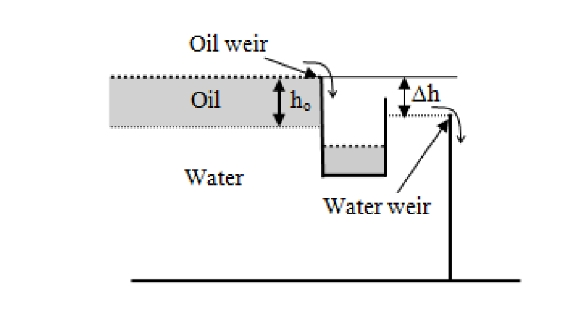
\includegraphics[width=0.5\columnwidth]{figs/i 4.jpeg}
        \caption{}
        \label{fig:placeholder}
    \end{figure}
 
    
    \begin{enumerate} \begin{multicols}{2}              
        \item $0.2 h_0$  
        \item $0.8 h_0$  
        \item $1.0 h_0$  
        \item $1.2 h_0$
    \end{multicols} \end{enumerate}              
    
    \hfill{\brak{\text{GATE PE 2016}}}
    
    \item The vertical lift performance \brak{VLP} and the inflow performance relationship \brak{IPR} curves are used to find the production operating conditions. If $P_{wf}$ is the flowing bottom-hole pressure and Q is the oil flow rate, select the CORRECT statement.
    \begin{figure}
        \centering
        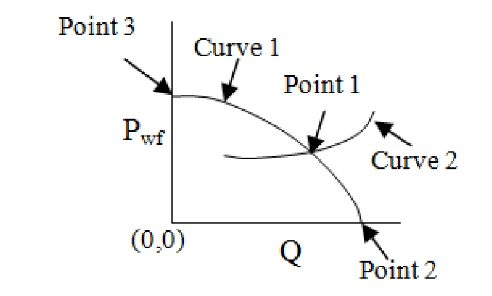
\includegraphics[width=0.5\columnwidth]{figs/i 5.jpeg}
        \caption{}
        \label{fig:placeholder}
    \end{figure}
    
    
    \begin{enumerate}               
        \item Point 3 is absolute open flow, Curve 1 is VLP curve.
        \item Point 2 is at reservoir pressure, Curve 2 is VLP curve.
        \item Point 1 is operating condition, Curve 2 is IPR curve.
        \item Point 2 is absolute open flow, Curve 1 is IPR curve.
 \end{enumerate}              
    
    \hfill{\brak{\text{GATE PE 2016}}}
    
    \item A ground station has a pump, which delivers a head of 1,000 m water. It is pumping oil of specific gravity 0.8 into a horizontal pipe of diameter 0.5 m with an average velocity of 2 m/s. The efficiency of the pump is 80\%. Density of water is 1,000 kg/m$^3$ and acceleration due to gravity is 9.8 m/s$^2$.
    
    The power required to operate the pump is \_\_\_\_\_ Mega Watts.
    
    \hfill{\brak{\text{GATE PE 2016}}}
    
    \item For a floating vessel, match the CORRECT pairs from Group 1 and Group 2 among the options given below. \brak{\text{B = Centre of buoyancy; G = Centre of gravity and M = Metacentre}}
    
   \begin{table}[h!]
\centering
\[
\begin{array}{|l|l|}
\hline
\textbf{Group 1} & \textbf{Group 2} \\
\hline
P. \; M \text{ is above G}      & I. \; \text{Stable equilibrium condition} \\
Q. \; M \text{ is below G}      & II. \; \text{Critically stable condition} \\
R. \; M \text{ coinciding with G} & III. \; \text{Unstable condition} \\
S. \; B \text{ is below G}      &  \\
\hline
\end{array}
\]
\caption{Matching of Group 1 and Group 2 conditions}
\label{tab:stability}
\end{table}

    
    \begin{enumerate} \begin{multicols}{2}              
        \item P-II, Q-III, R-I and S-II
        \item P-I, Q-III, R-II and S-I
        \item P-III, Q-I, R-II and S-III
        \item P-I, Q-II, R-III and S-I
    \end{multicols} \end{enumerate}              
    
    \hfill{\brak{\text{GATE PE 2016}}}
    
    \item Match the following
    
    \begin{table}[h!]
\centering
\[
\begin{array}{|l|l|}
\hline
\textbf{Group 1} & \textbf{Group 2} \\
\hline
P. \; \text{Master valve}   & I. \; \text{Drill stem testing tool} \\
Q. \; \text{Breather valve} & II. \; \text{Heater-treater} \\
R. \; \text{Tester valve}   & III. \; \text{Christmas tree} \\
S. \; \text{Dump valve}     & IV. \; \text{Positive displacement motor} \\
                            & V. \; \text{Storage tank} \\
\hline
\end{array}
\]
\caption{Matching of Group 1 and Group 2 components}
\label{tab:valves}
\end{table}

    
    \begin{enumerate} \begin{multicols}{2}              
        \item P-III, Q-V, R-II and S-I
        \item P-III, Q-V, R-I and S-IV
        \item P-II, Q-III, R-I and S-V
        \item P-I, Q-III, R-II and S-IV
    \end{multicols} \end{enumerate}              
    
    \hfill{\brak{\text{GATE PE 2016}}}
    
    \item A core, with a length of 10 cm, breadth of 4 cm and width of 4 cm, weighs 282.4 g in its dry form. The core is then saturated 100\% with brine of density 1.1 g/cm$^3$. The brine saturated core weighs 300 g.
    
    The porosity of this core sample is \_\_\_\_\_\%.
\begin{figure}
    \centering
    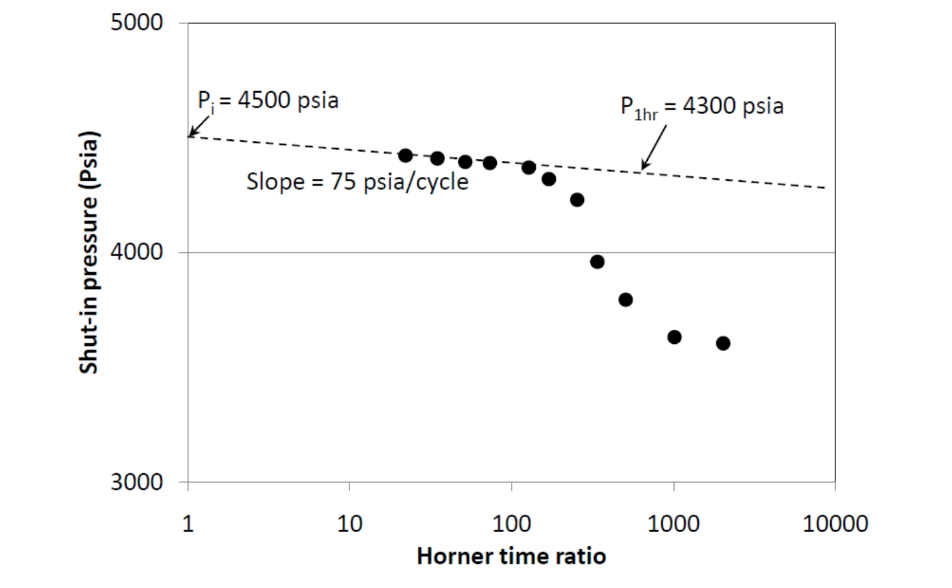
\includegraphics[width=0.5\columnwidth]{figs/i 6.jpeg}
    \caption{}
    \label{fig:placeholder}
\end{figure}
    \hfill{\brak{\text{GATE PE 2016}}}
    
    \item During a production test in an oil reservoir, the oil production rate is 200 STB/day. The producing gas oil ratio \brak{GOR} is 800 SCF/STB and dissolved GOR is 200 SCF/STB. The formation volume factor of gas is 0.01 ft$^3$/SCF and the formation volume factor of oil is 1.2 reservoir-bbl/STB.
    
    The down-hole GOR is \_\_\_\_\_ ft$^3$/reservoir-bbl.
    
    \hfill{\brak{\text{GATE PE 2016}}}
    
    \item A productivity test was conducted on a single-phase crude oil well. The well is capable of producing 100 STB/day at a flowing bottom-hole pressure of 1000 psig. The 24-hour shut-in static pressure is found to be 1500 psig.
    
    The maximum oil flow rate ($Q_{max}$) is \_\_\_\_\_ STB/day.
    
    \hfill{\brak{\text{GATE PE 2016}}}
    
    \item An oil well of wellbore radius 0.5 ft is shown to develop a skin due to formation damage. The damaged zone radius is 2.25 ft around the well. The formation permeability is 300 md and the permeability of the damaged zone is 100 md.
    
    The effective well bore radius for this well is \_\_\_\_\_ ft.
    
    \hfill{\brak{\text{GATE PE 2016}}}
    
    \item A producing well has a shut-in tubing pressure of 3,950 psig for crude oil of specific gravity 0.69. [1 g/cm$^3$ = 8.33 ppg]
    
    The kill fluid density for a workover job at 11,600 ft \brak{TVD} is \_\_\_\_\_ ppg.
    
    \hfill{\brak{\text{GATE PE 2016}}}
    
    \item For a water-flood operation in a one-dimensional reservoir, the following data are given. Porosity, $\phi = 0.25$; Cross-sectional area, $A = 25,000$ ft$^2$; Horizontal distance between the vertical production and injection well = 600 ft; Water injection rate, $i_w = 900$ bbl/day; Slope of fractional flow curve at shock front water saturation = 1.97; Water formation volume factor = 1.0 bbl/STB.
    
    [1 bbl = 5.615 ft$^3$]
    
    The cumulative water volume injected at breakthrough is \_\_\_\_\_ $\times 10^5$ bbl.
    
    \hfill{\brak{\text{GATE PE 2016}}}
    
    \item A heavy oil reservoir is being flooded with a line drive \brak{\text{assume one-dimensional flooding}}. The fractional flow of water is found to be 0.75 bbl/bbl at water saturation ($S_w$) of 60\%. A polymer solution with twice the viscosity of water is used as displacing phase. Assume the relative permeability curves for water flooding and polymer flooding are the same.
    
    The fractional flow of polymer solution at a saturation of 60\% is \_\_\_\_\_ bbl/bbl.
    
    \hfill{\brak{\text{GATE PE 2016}}}
\end{enumerate}              


\vspace{0.5cm}
\begin{center}
\textbf{\large --- END OF THE QUESTION PAPER ---}
\end{center}
\end{document}